\chapter{Dataset}
\label{chap:dataset}

A crucial part in the development of deep learning model is the dataset used for training. There are several datasets proposed in the literature for logo detection and recognition, however, some of them like BelgaLogos \cite{neumann2002integration} lack of variety in the number of classes and have a small number of images. For this reason, some works aimed to construct some larger dataset, such as WebLogo-2M \cite{su2017weblogo} or Logos in the wild \cite{tuzko2017open}. The issue with these types of large scale dataset is that they are automatically collected and labeled, leading to some noise in the target label.

A list of datasets proposed in the literature is given by Li et al. in SeeTek \cite{li2022seetek}, shown in \autoref{table:logo-datasets}.

\begin{table}
    \begin{center}
        \begin{tabular}{c || c | c | c | c | c |c} 
            \hline
            \textbf{Dataset} & \textbf{Logos} & \textbf{Images} & \textbf{Annotation} & \textbf{Noisy} & \textbf{Public} & \textbf{Scalability} \\
            \hline
            \hline
            TopLogo-10 \cite{su2017deep} & 10 & 700 & Object-Level & no & yes & Weak \\ 
       \hline
           BelgaLogos \cite{joly2009logo} & 37 & 10,000 & Object-Level & no & yes & Weak \\ 
       \hline
           FlickrLogos-32 \cite{romberg2011scalable} & 32 & 8,240 & Object-Level & no & yes & Weak \\ 
       \hline
           FlickrLogos-47 \cite{romberg2011scalable} & 47 & 8,240 & Object-Level & no & yes & Weak \\ 
       \hline
           Logo-NET \cite{hoi2015logo} & 160 & 73,414 & Object-Level & no & yes & Weak \\ 
       \hline
           WebLogo-2M \cite{su2017weblogo} & 194 & 2,190,757 & Image-Level & yes & yes & Medium \\ 
       \hline
           QMUL-OpenLogo \cite{su2018open} & 352 & 27,083 & Image-Level & no & yes & Medium \\ 
       \hline
           Logos in the wild \cite{tuzko2017open} & 871 & 11,054 & Object-Level & yes & yes & Medium \\ 
       \hline
           BLAC \cite{bastan2019large} & 2,800 & 6,200 & Object-Level & no & no & Medium \\ 
       \hline
           LogoDet-3K \cite{wang2022logodet} & 3,000 & 158,652 & Object-Level & no & yes & Strong \\ 
       \hline
           PL8K \cite{li2022seetek} & 7,888 & 3,017,146 & Object-Level & no & no & Strong \\ 
           \hline
       
           \end{tabular}
    \end{center}
    
    \caption{Statistics and characteristics of existing logo detection datasets \cite{li2022seetek}.}
    \label{table:logo-datasets}
\end{table}

Some logos datasets like LogoDet-3K and PL8K are considered more robust for what concern the annotation of the images (noisy column in \autoref{table:logo-datasets}). In particular, each image of LogoDet-3K is manually examined and
reviewed, this guarantees high-quality annotations.

In the face of this, the only two large-scale and non-noisy datasets of \autoref{table:logo-datasets} are LogoDet-3K and PL8K. However, only LogoDet-3K is publicly available, thus being the only viable choice as the target dataset to use for the experiments of this thesis (see \autoref{chap:experiments}).


\section{LogoDet-3K: dataset description}
\label{sec:logodet-desc}
LogoDet-3K consists of 3,000 logo classes,
158,652 images and 194,261 logo objects. The objects correspond to the bounding boxes in each image, and since an image can contain more than one logo, the number of objects is grater than the number of images. 
The dataset is divided into nine categories, each category contains several brands and for each brand there is a set of images of that brand. The \autoref{table:logodet3k-category-statistics} shows the number of brands, images and objects for each category.

In this context, brand is intended as logo class. In fact, the same brand can have multiple versions of logos, for example, a symbolic logo and a textual logo. These type of logos are treaded as different classes in the LogoDet-3K dataset, a suffix such as '\textit{brand}-1' and '\textit{brand}-2' is used to deal with these cases. An example is given in \autoref{fig:logos-suffix}.
It is important to point out how an image can contain multiple logo objects and the objects in the same image are not necessary of the same class.


\begin{figure}%
	\centering

    \begin{center}
        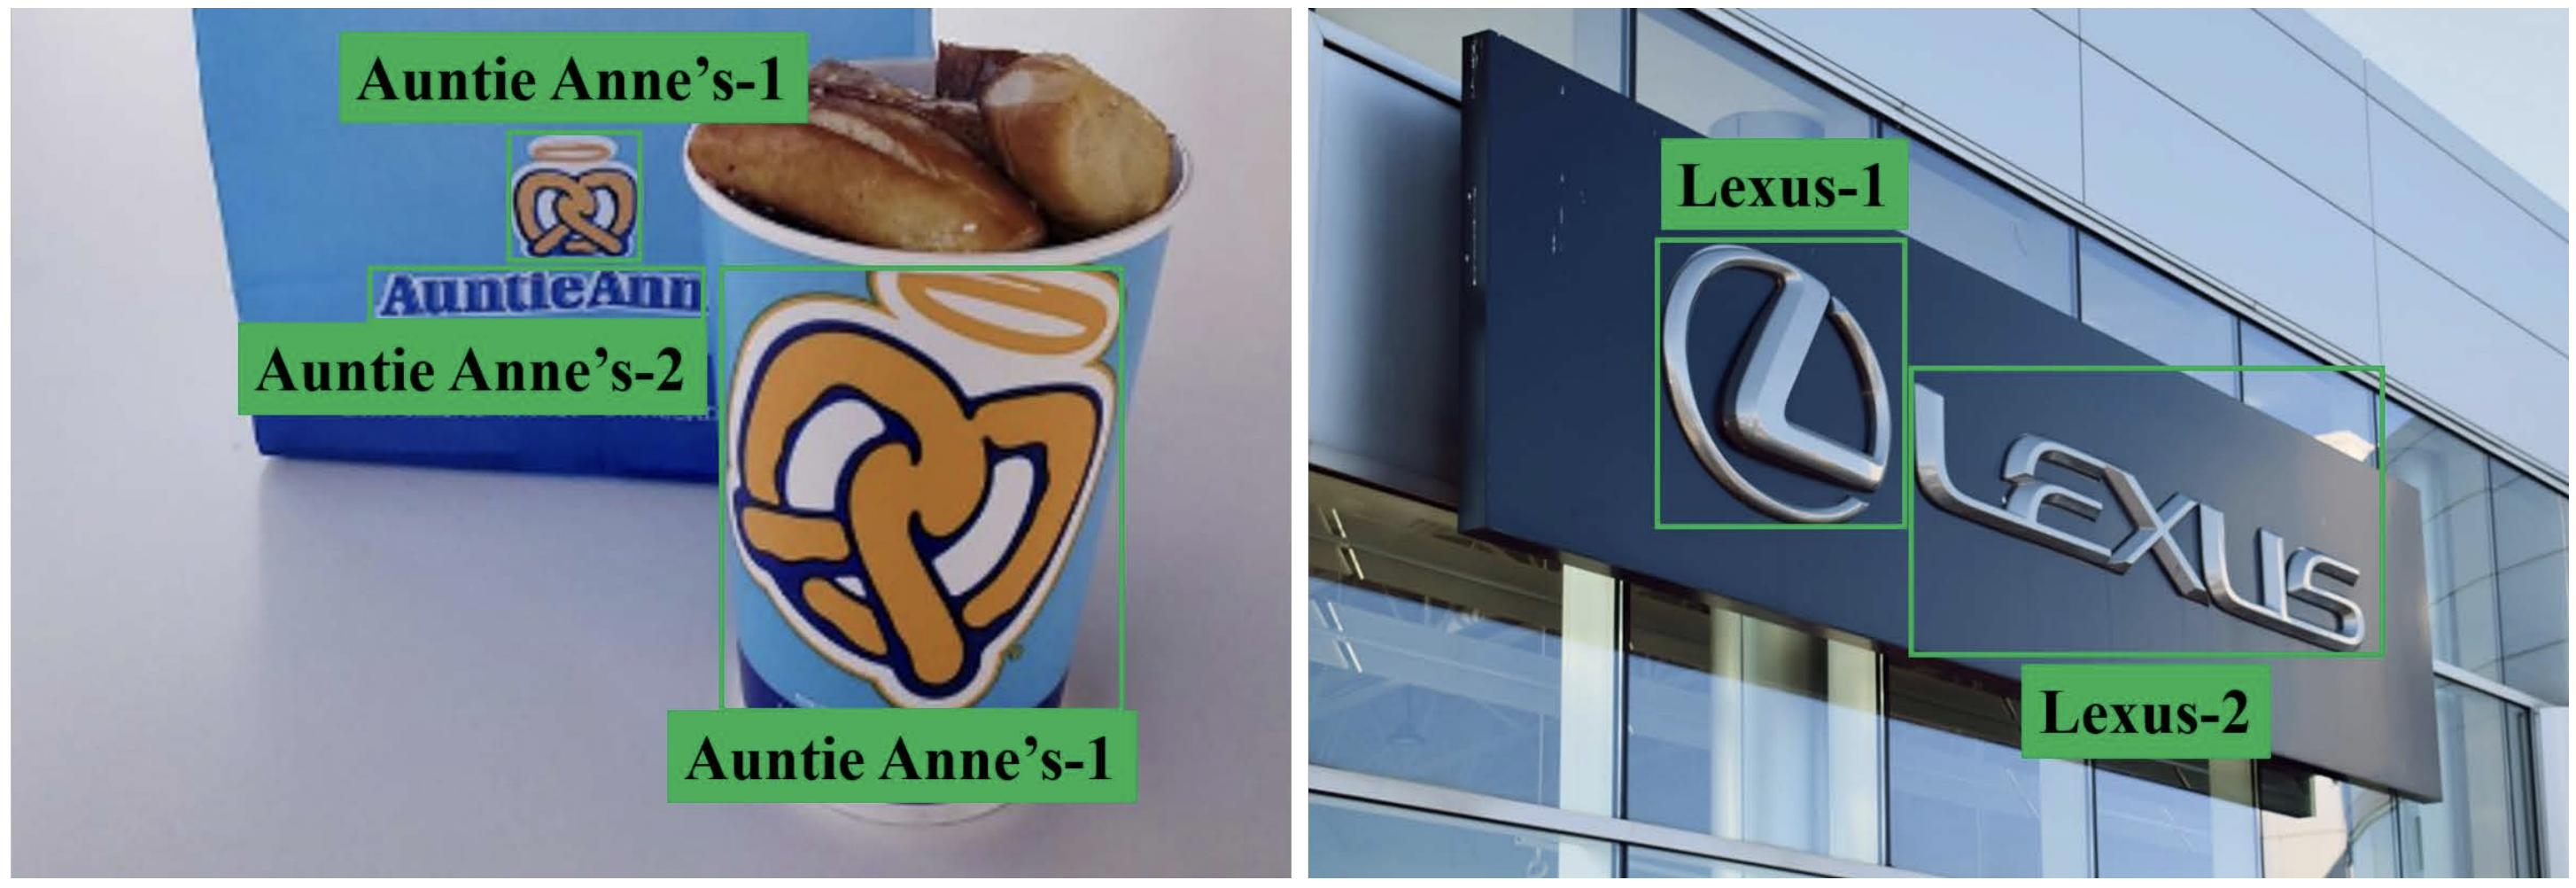
\includegraphics[width=\columnwidth]{images/logos-suffix.png}
    \end{center}
	\caption{Same brand treated as different class using the suffixes '-1' and '-2' \cite{wang2022logodet}.}%
	\label{fig:logos-suffix}%
\end{figure}

\begin{table}
    \centering
    \begin{tabular}{c | c  c  c } 
     \hline
     \textbf{Category} & \textbf{Brand} & \textbf{Images} & \textbf{Objects} \\
     \hline
    Food & 932 & 53,350 & 64,276 \\ 
    Clothes & 604 & 31,266 & 37,601 \\ 
    Necessities & 432 & 24,822 & 30,643 \\ 
    Electronic & 224 & 9,675 & 12,139 \\ 
    Transportation & 213 & 10,445 & 12,791 \\ 
    Leisure & 111 & 5,685 & 6,573 \\ 
    Sports & 66 & 3,953 & 5,041 \\ 
    Medical & 47 & 3,945 & 5,185 \\ 
    Others & 371 & 15,513 & 20,016 \\ 
    \hline
    Total & 3,000 & 158,652 & 194,261 \\ 

    \end{tabular}
    \caption{Brand, images and objects number for each category of LogoDet-3K dataset \cite{wang2022logodet}.}
    \label{table:logodet3k-category-statistics}
\end{table}

\subsection{Dataset statistics}
The \autoref{fig:logodet-dist} shows the distribution of the number of objects for each logo class.
\begin{figure}[ht]
	\centering

    \begin{center}
        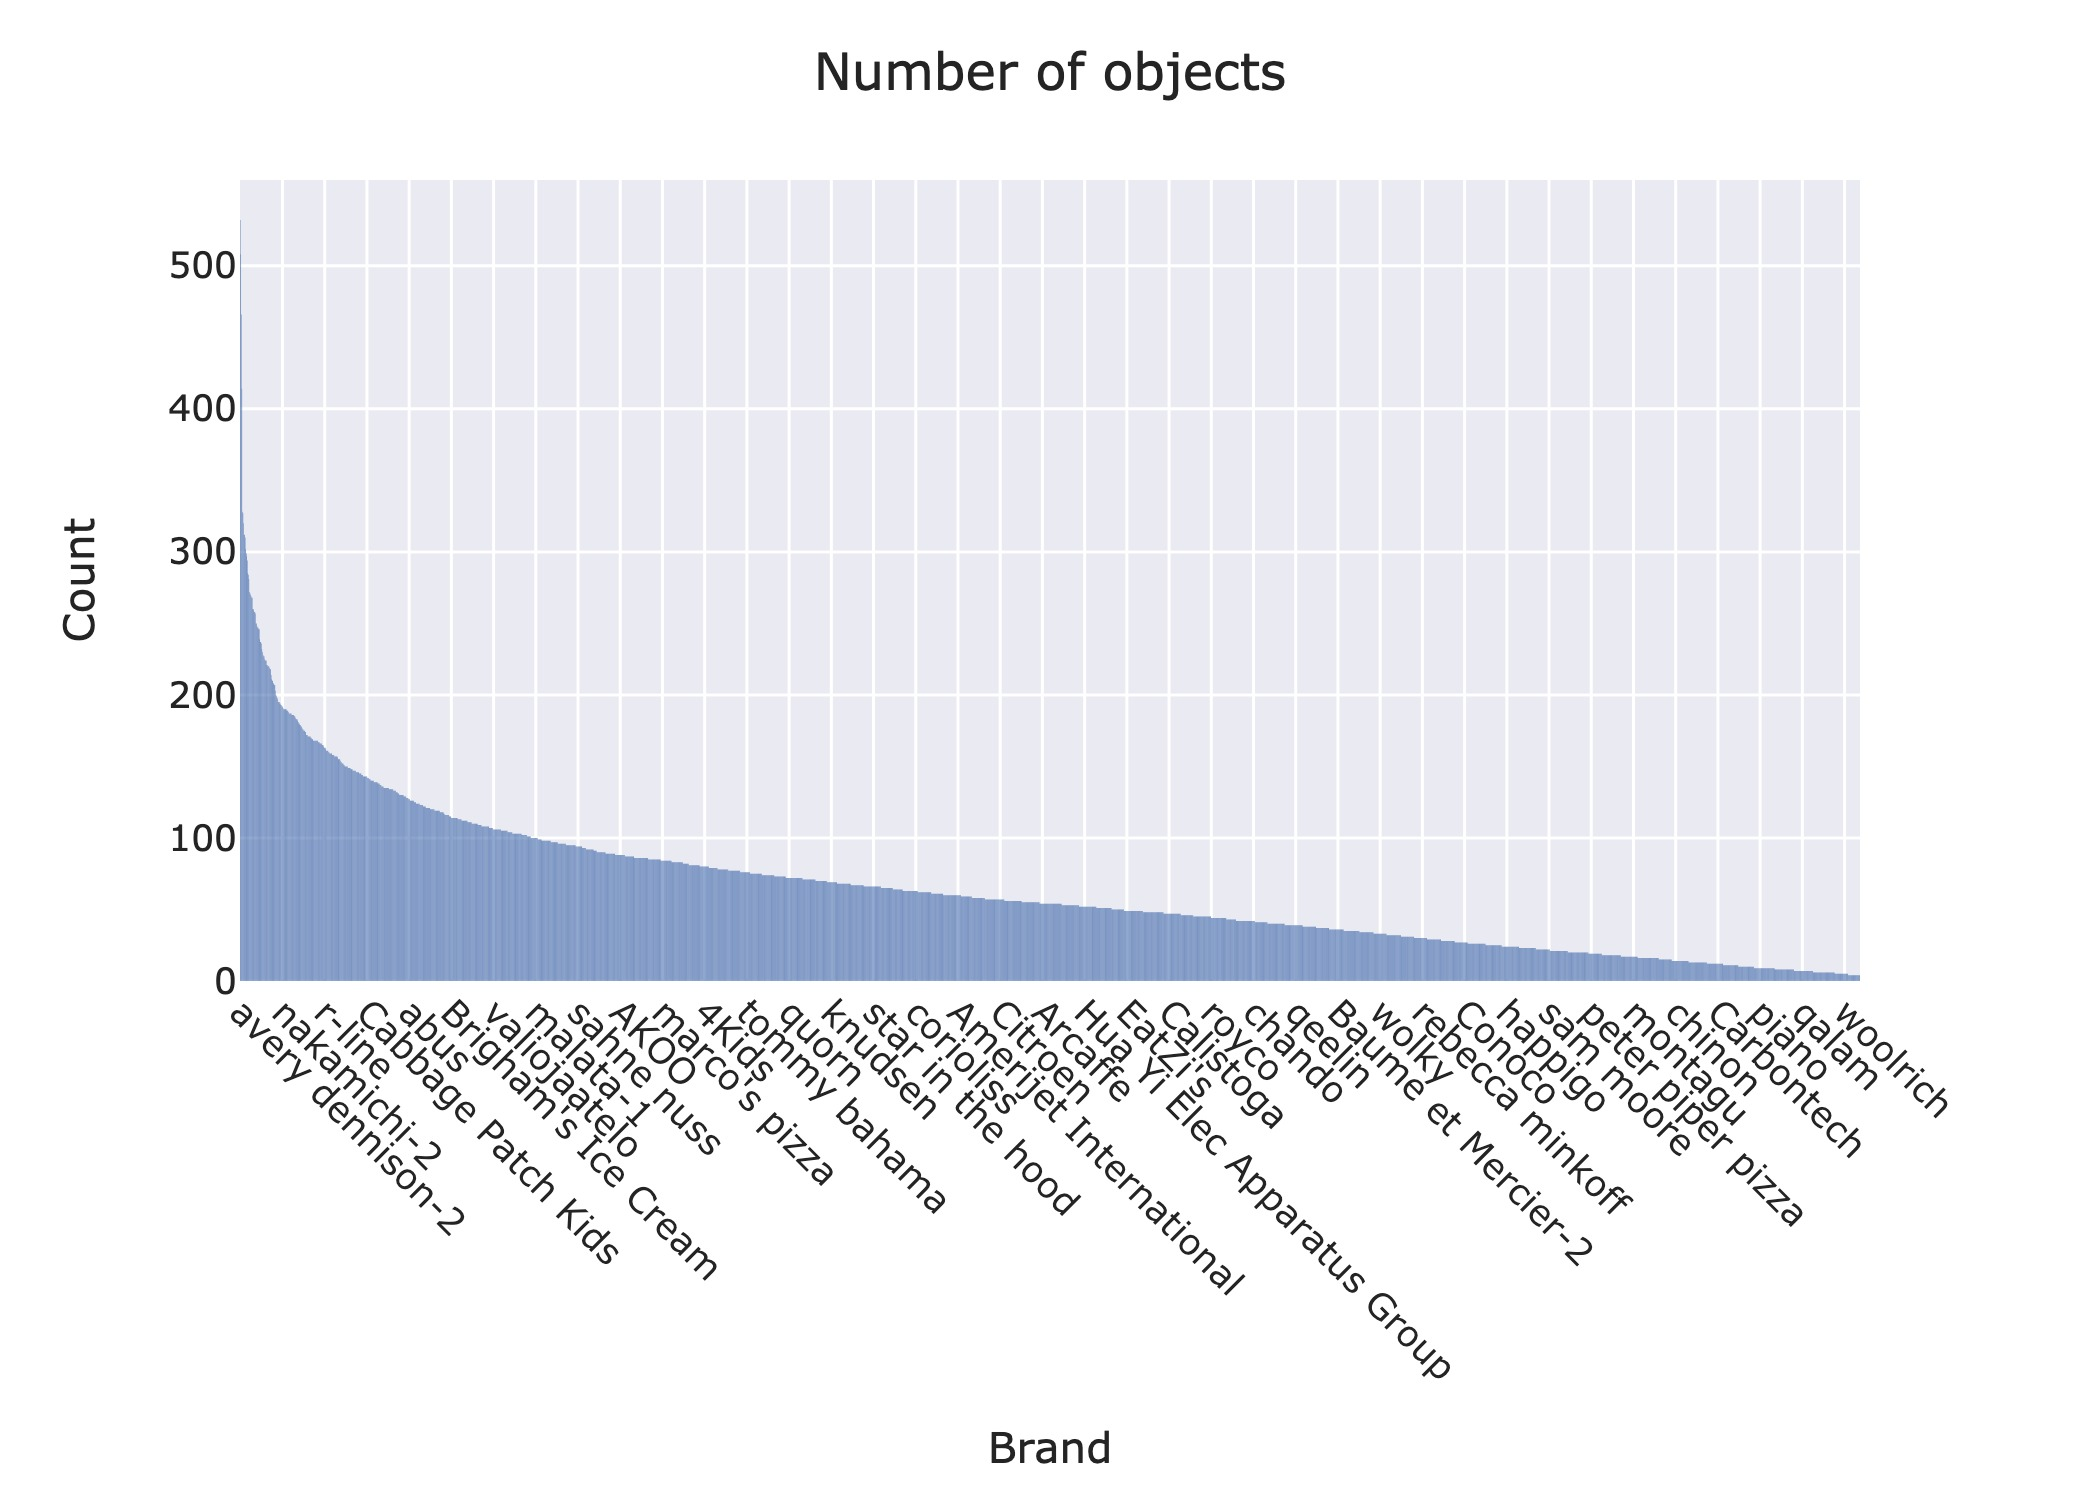
\includegraphics[width=\columnwidth]{images/freq.jpeg}
    \end{center}
	\caption{Number of objects in LogoDet-3K for each class.}%
	\label{fig:logodet-dist}%
\end{figure}


The main issue of LogoDet-3K is the low number of objects for some classes. Analyzing the boxplot in \autoref{fig:logodet-boxplot} and the statistics of \autoref{table:logodet3k-quartile} emerges how the 25\% of the classes have a number of images less or equal to 27. Moreover, half of the classes have a number of images less or equal to 54. This is the main issue with this dataset: since several classes have a low number of images, it could be challenging for the model to correctly predict these classes.  



\begin{figure}[ht]
	\centering

    \begin{center}
        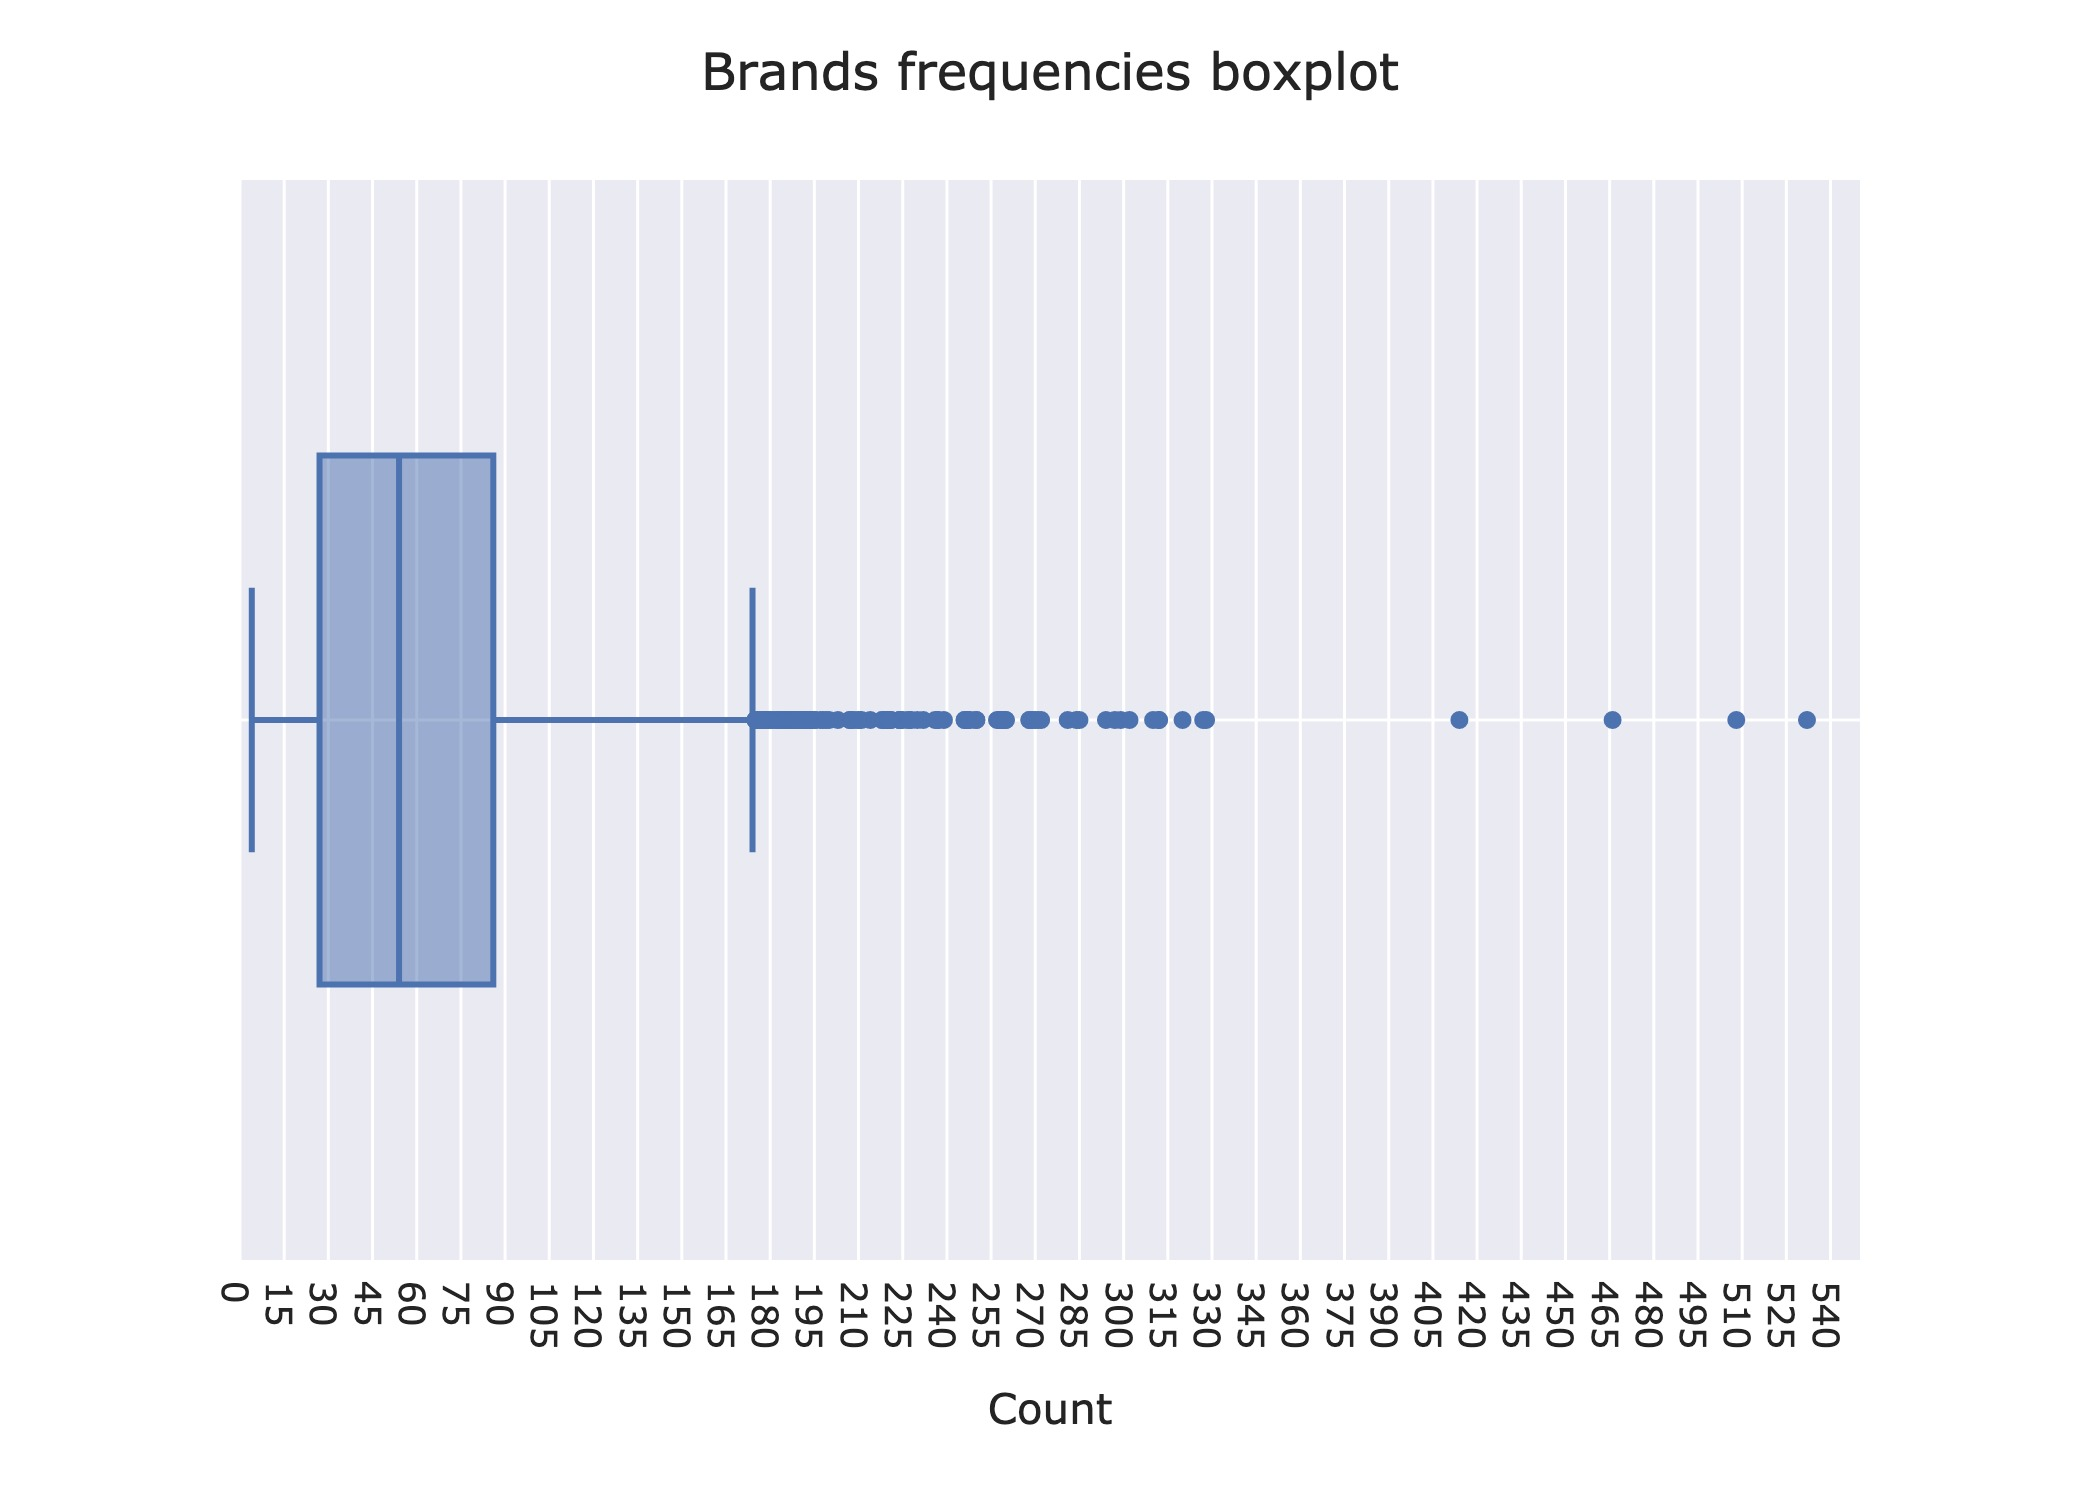
\includegraphics[width=\columnwidth]{images/box_plot.jpeg}
    \end{center}
	\caption{Boxplot of the number of objects in LogoDet-3K for each class.}%
	\label{fig:logodet-boxplot}%
\end{figure}


\begin{table}[ht]
    \centering
    \begin{tabular}{c  c  c  c } 
     \hline
     \multicolumn{4}{c}{LogoDet-3K statistics}\\
     \hline
     \textbf{$Q_1$} & \textbf{$Q_2$} & \textbf{$Q_3$} & \textbf{$Q_4$} \\
     \hline
     27 & 54 & 86 & 532 \\
    \end{tabular}
    \caption{Quartiles relative to the number of objects for each brand in LogoDet-3K dataset.}
    \label{table:logodet3k-quartile}
\end{table}

\section{Inconsistencies in the dataset}
The LogoDet-3K dataset is available in the GitHub repository\footnote{PyCIL GitHub repository: \href{https://github.com/G-U-N/PyCIL}{https://github.com/G-U-N/PyCIL}} mentioned in the original paper \cite{wang2022logodet}. The dataset is provided in 9 sub-directories corresponding to each category described in \autoref{sec:logodet-desc}, and for each category there are several sub-directories corresponding to each logo class (brand). Inside each brand's folder there are the images and the metadata containing the annotation regarding the bounding box coordinates and the actual class of the logo, since an image can contain logo of different classes. The dataset structure can be summarized as follows:\\

\begin{forest}
    for tree={%
      folder,
      grow'=0,
      fit=band,
    }
    [LogoDet-3K
        [Food]
        [Clothes]
        [Necessities]
        [Electronic]
        [Transportation]
        [Leisure]
        [Sports]
        [Medical]
        [Others
            [avery dennison-1
                [\underline{1.jpg}]
                [\underline{1.xml}]
                [...]
            ]
            [avery dennison-1
                [\underline{1.jpg}]
                [\underline{1.xml}]
                [...]
            ]  
            [...]
        ]
    ]
\end{forest}\\
Although the number of subdirectories in each category sums to 3,000 (i.e. the number of classes of the dataset), using the dataset provided in the GitHub repository, when analyzing the metadata of the '.xml' files, the number of the uniques logo classes is 2,993. This is a discrepancy in the dataset between what is described in the original paper and the dataset downloaded from the GitHub repository.

Another issue related with this dataset is that some images contain errors regarding the annotation in the metadata. For example, the two images:
\begin{enumerate}
    \item \code{Others/avery dennison-1/27.jpg} labeled in \code{Others/avery dennison-1/27.xml}
    \item \code{Others/avery dennison-2/56.jpg} labeled in \code{Others/avery dennison-2/56.xml}
\end{enumerate}
are labeled as shown in \autoref{fig:logodet-error}. 


\begin{figure}%
	\centering
	\subfloat[\centering Image \code{Others/avery dennison-1/27.jpg}]{{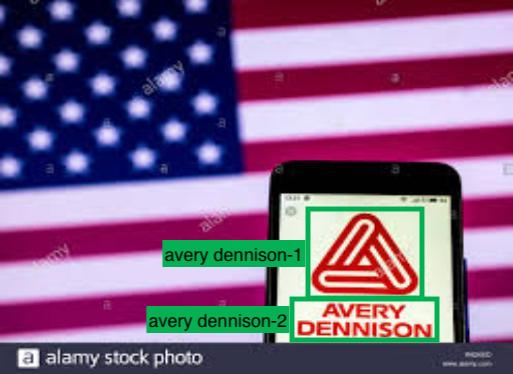
\includegraphics[width=0.45\textwidth]{images/image-27.png} }}%
	\hfill
	\subfloat[\centering Image \code{Others/avery dennison-2/56.jpg}]{{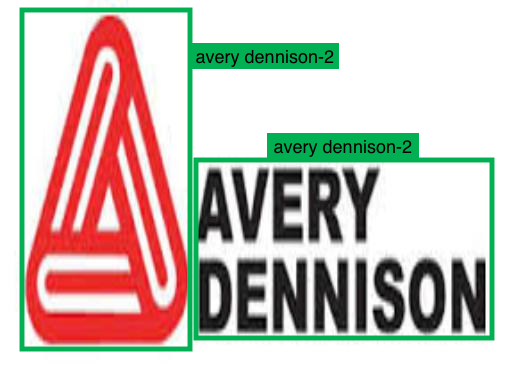
\includegraphics[width=0.45\textwidth]{images/image-56.png} }}%
	\caption{Example of errors in the annotation of the images.}
	\label{fig:logodet-error}%
\end{figure}

From \autoref{fig:logodet-error} it is clear how the labeling is not consistent between the two images. In the image \code{Others/avery dennison-1/27.jpg} the logos are treated (correctly) as different classes. On the other hand, in the image \code{Others/avery dennison-2/56.jpg} the two logos are treated as the same class.

The vast majority of images are labeled correctly, however, especially for those classes related to the same brand and distinguished by the use of suffixes, some errors such as the one just discussed are present.